\documentclass[main]{subfiles}
\begin{document}

\section*{Lecture 19 // Oct 27 // SU(2)-Character Varieties}
\addcontentsline{toc}{section}{Lecture 19 -- SU(2)-Character Varieties}

This week, we'll return to our discussion of the $\SU(2)$ character variety. We briefly mentioned this perspective when we discussed the critical points of the CS functional, but we haven't done any examples nor explicit calculations yet. Recall that we can study the fundamental group of a $3$-manifold by considering instead the image of $\pi_1(Y)$ under some homomorphism to a simpler group, $\SU(2)$.

\begin{definition}
The Character Variety of a $3$-manifold is
\[
\mc{R}(Y) = \left\{\begin{array}{c}\SU(2) \text{ representations} \\ \text{of } \pi_1(Y)\end{array}\right\}\Big/\!\sim
\]
where $\rho_0\sim\rho_1$ iff $\rho_1 = g^{-1}\cdot\rho_0\cdot g$.
\end{definition}

Today, we'll discuss Fintushel-Stern's computation of IFH of Brieskorn spheres $\Sigma(a_1,\dots,a_n)$. Recall that if the set of critical points of $\CS(Y)$ is not discrete, we need to perturb the functional to get a discrete set. With this in mind, we'll do examples of both situations: when $\mc{R}$ is discrete and when $\mc{R}$ has higher-dimensional components.

On Thursday, we'll discuss the common idea of viewing one's favorite gauge theory as the categorification of something. For $\mathrm{IFH}_\ast$, this ``something'' is the Casson invariant:
\[
\frac{1}{2}\chi\big(H_\ast(C(Y))\big) = \lambda(Y).
\]

\subsection*{Examples of $\SU(2)$ character varieties}

First, let's recall some facts about $\SU(2)$.

\begin{enumerate}
\item $\SU(2) = \left\{\begin{pmatrix}\alpha & -\bar\beta \\ \beta & \bar\alpha\end{pmatrix} \,\Big|\, \alpha,\beta\in\mathbb{C},\ |\alpha|^2+|\beta|^2=1\right\}$ is diffeomorphic to $S^3$. Going forward, we'll think of $\SU(2)$ as $S^3$, which we'll draw $1$-dimension down as $S^2$.

\item $\SU(2)$ has many $S^1$ subgroups, which are all conjugate to each other and sweep out $\SU(2)$. They are all disjoint except at $\pm I$. I.e., every element of $\SU(2)$ is conjugate to some diagonal matrix $\begin{pmatrix}e^{i\theta} & 0\\ 0 & e^{-i\theta}\end{pmatrix}$ which is unique up to the sign of $\theta$.
\begin{center}
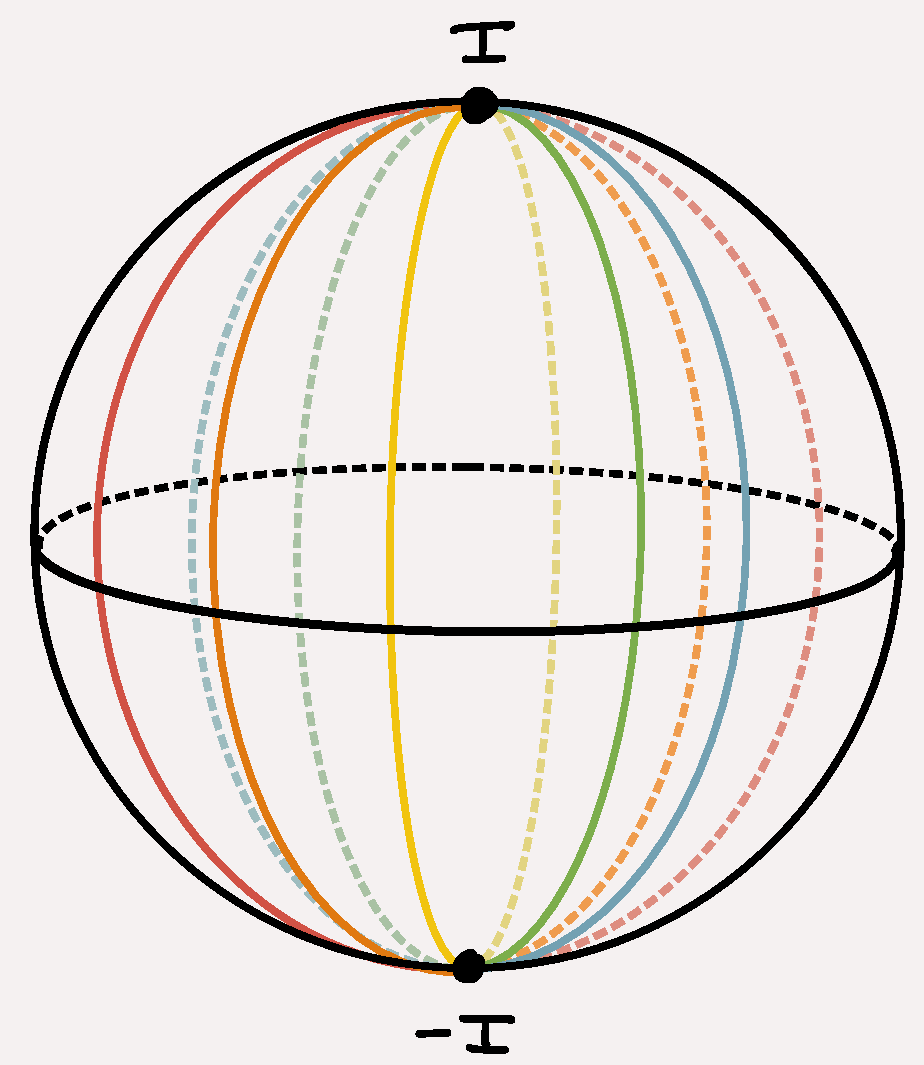
\includegraphics[width=0.4\linewidth]{figures/fig_lec19_su2_subgroups.png}
\end{center}

\item For $A\in\SU(2)$, $\mathrm{Tr}(A)$ is a complete invariant up to conjugation: if $A$ and $B$ are conjugate, $\mathrm{Tr}(A)=\mathrm{Tr}(B)$. Each conjugacy class is a $2$-sphere $S^2$ parameterized by the value of $\mathrm{tr}$. For $\theta\in[0,\pi]$, we will speak of the conjugacy class of $[\theta]$ to mean the conjugacy class of $\begin{pmatrix}e^{i\theta} & 0\\ 0 & e^{-i\theta}\end{pmatrix}$, where
\[
\theta = \cos^{-1}\left(\frac{1}{2}\mathrm{Tr}\begin{pmatrix}e^{i\theta} & 0\\ 0 & e^{-i\theta}\end{pmatrix}\right).
\]
\begin{center}
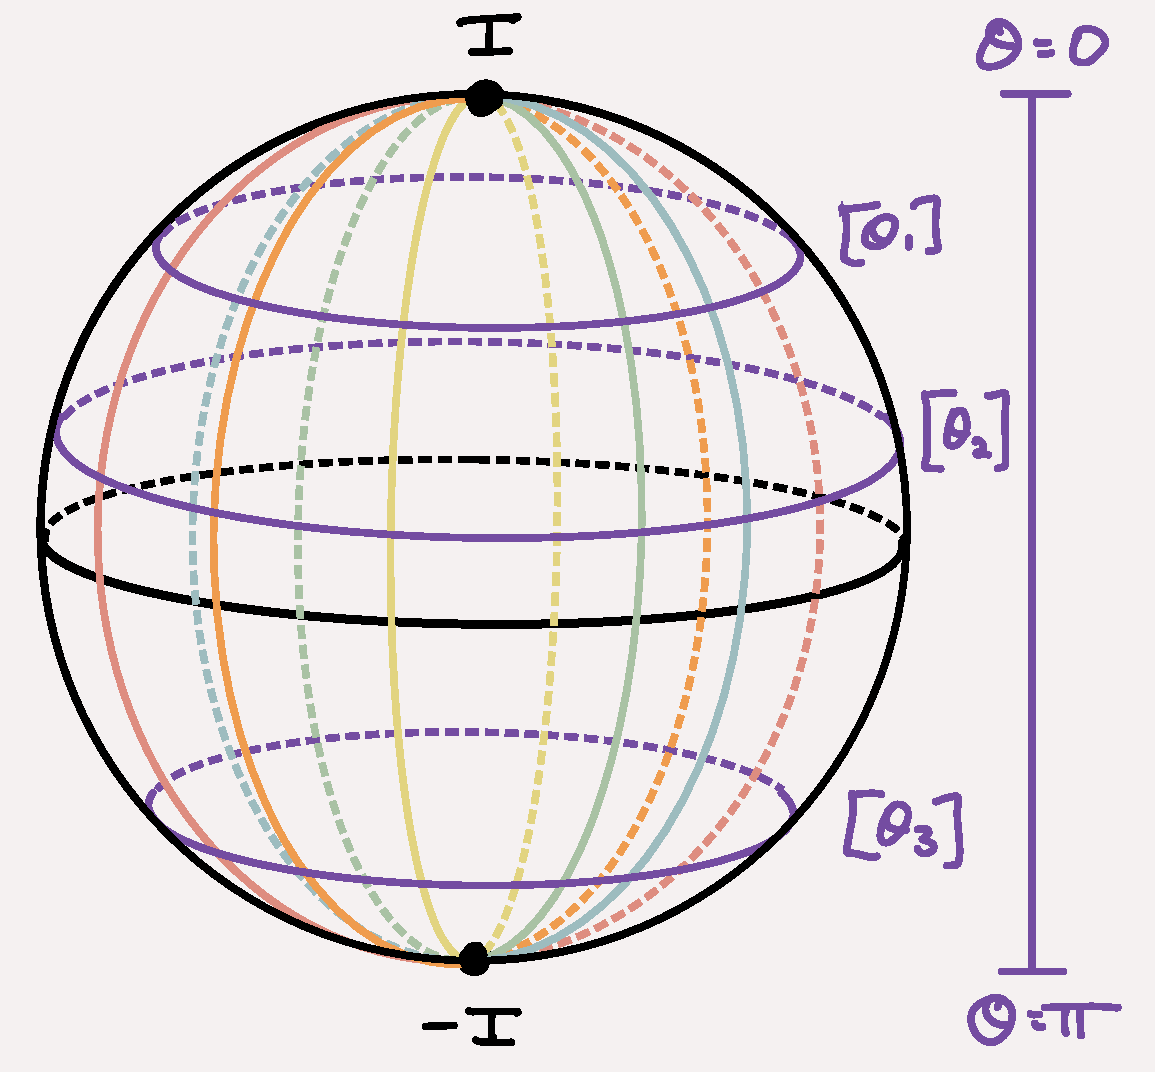
\includegraphics[width=0.5\linewidth]{figures/fig_lec19_conj_classes.png}
\end{center}
\end{enumerate}

We can now compute the representation variety of a Brieskorn sphere $\Sigma(a_1,\dots,a_n)$, where the $a_i$ are coprime.

\begin{definition}
The Brieskorn spheres $\Sigma(a_1,\dots,a_n)$ are $\mathbb{Z}\mathrm{HS}^3$'s constructed as follows:
\begin{enumerate}
\item Solve the linear equation
\[
\left(\prod_{i=1}^n a_i\right)\left(\sum_{i=1}^n\frac{b_i}{a_i}\right) = 1
\]
for a set $\{b_1,\dots,b_n\}\in\mathbb{Z}^n$.
\item Surger $S^2\times S^1$ along $n$ longitudinal fibres with surgery coefficients $\left\{\frac{a_i}{b_i}\right\}_{i=1}^n$.
\end{enumerate}
E.g., punch out $n$ longitudinal $S^1$ factors to get $n$ $S^1\times S^1$ boundary components. Let $\mathrm{pt}\times S^1$ in $S^1\times S^2$ be homologous to $\mathrm{pt}\times S^1$ in $S^2\times S^1$, and $a/b$ be the class $a[S^1\times\mathrm{pt}]+b[\mathrm{pt}\times S^1]$. To each component, reglue $S^1\times D^2$ so that $[\partial D^2]\mapsto a[S^1\times\mathrm{pt}]+b[\mathrm{pt}\times S^1]$.
\end{definition}

\begin{center}
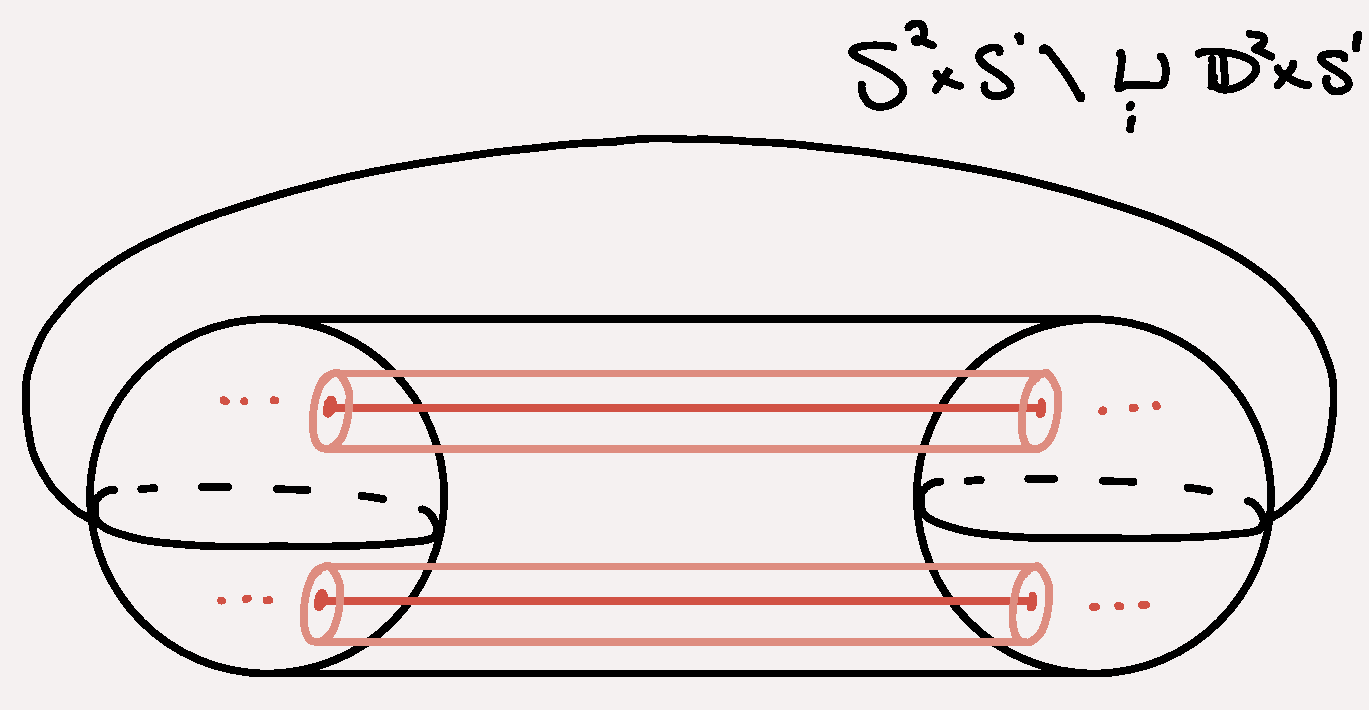
\includegraphics[width=0.55\linewidth]{figures/fig_lec19_punctured.png}
\hfill
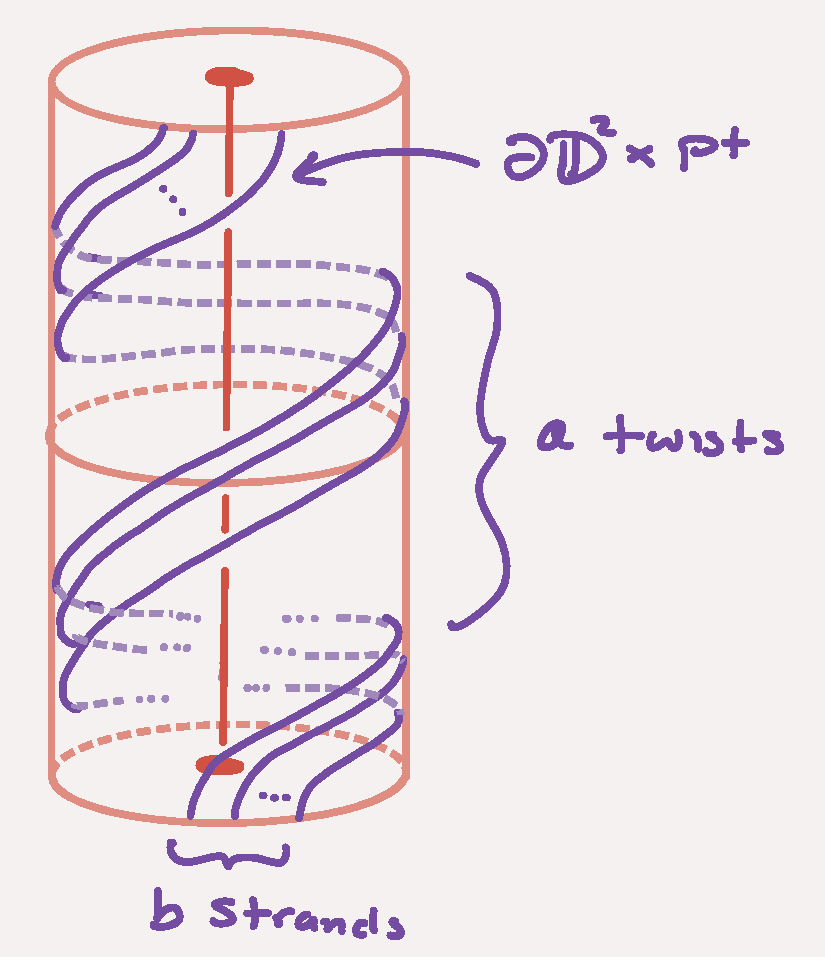
\includegraphics[width=0.25\linewidth]{figures/fig_lec19_twists.png}
\end{center}

This gives the following surgery description:
\begin{center}
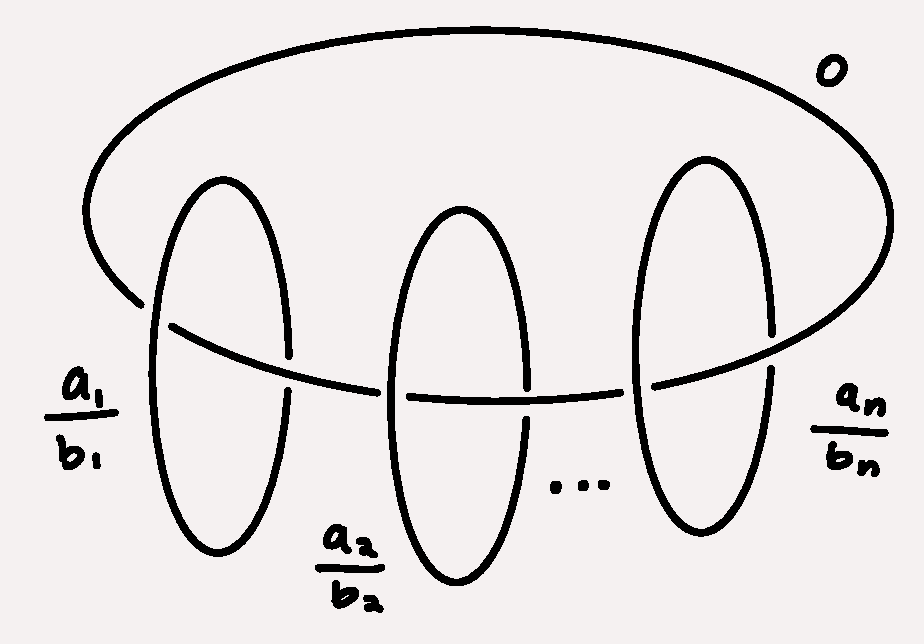
\includegraphics[width=0.45\linewidth]{figures/fig_lec19_surgery_link.png}
\end{center}

\begin{remark}
Sanity check for coefficients:
\begin{center}
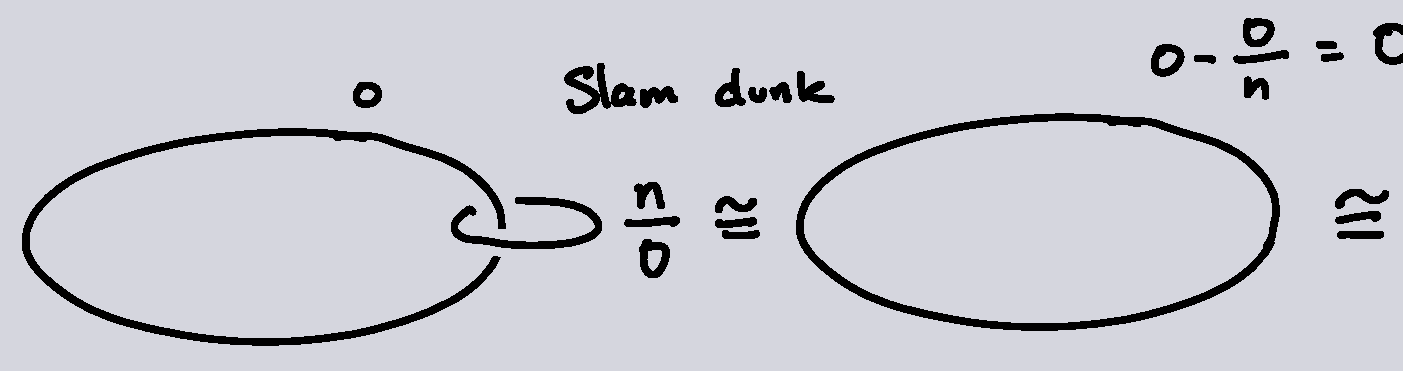
\includegraphics[width=0.6\linewidth]{figures/fig_lec19_slamdunk.png}
\end{center}
$S^2\times S^1$, so
\[
n\mapsto S^1\times\mathrm{pt}\subset S^2\times\mathrm{pt}, \qquad 0\mapsto \mathrm{pt}\times S^1\subset \mathrm{pt}\times S^1.
\]
\end{remark}

Of course, the $\{a_1,\dots,a_n\}$ do not uniquely determine a $3$-manifold. However, if we demand that the $3$-manifold is a $\mathbb{Z}\mathrm{HS}^3$, solving the equation above gives a set $\{b_i\}_{i=1}^n$, which is not necessarily unique, but one can show that they define the same $3$-manifold. (This notion of equivalency can be pasted over to equivalency of the sets $\{b_i\}$.)

To get the character variety, we first must compute the fundamental group. The generators are $x_1,\dots,x_n,h$, where the $x_1,\dots,x_n$ are loops about the meridional generator of each fibre and $h$ is the longitudinal direction.
\begin{center}
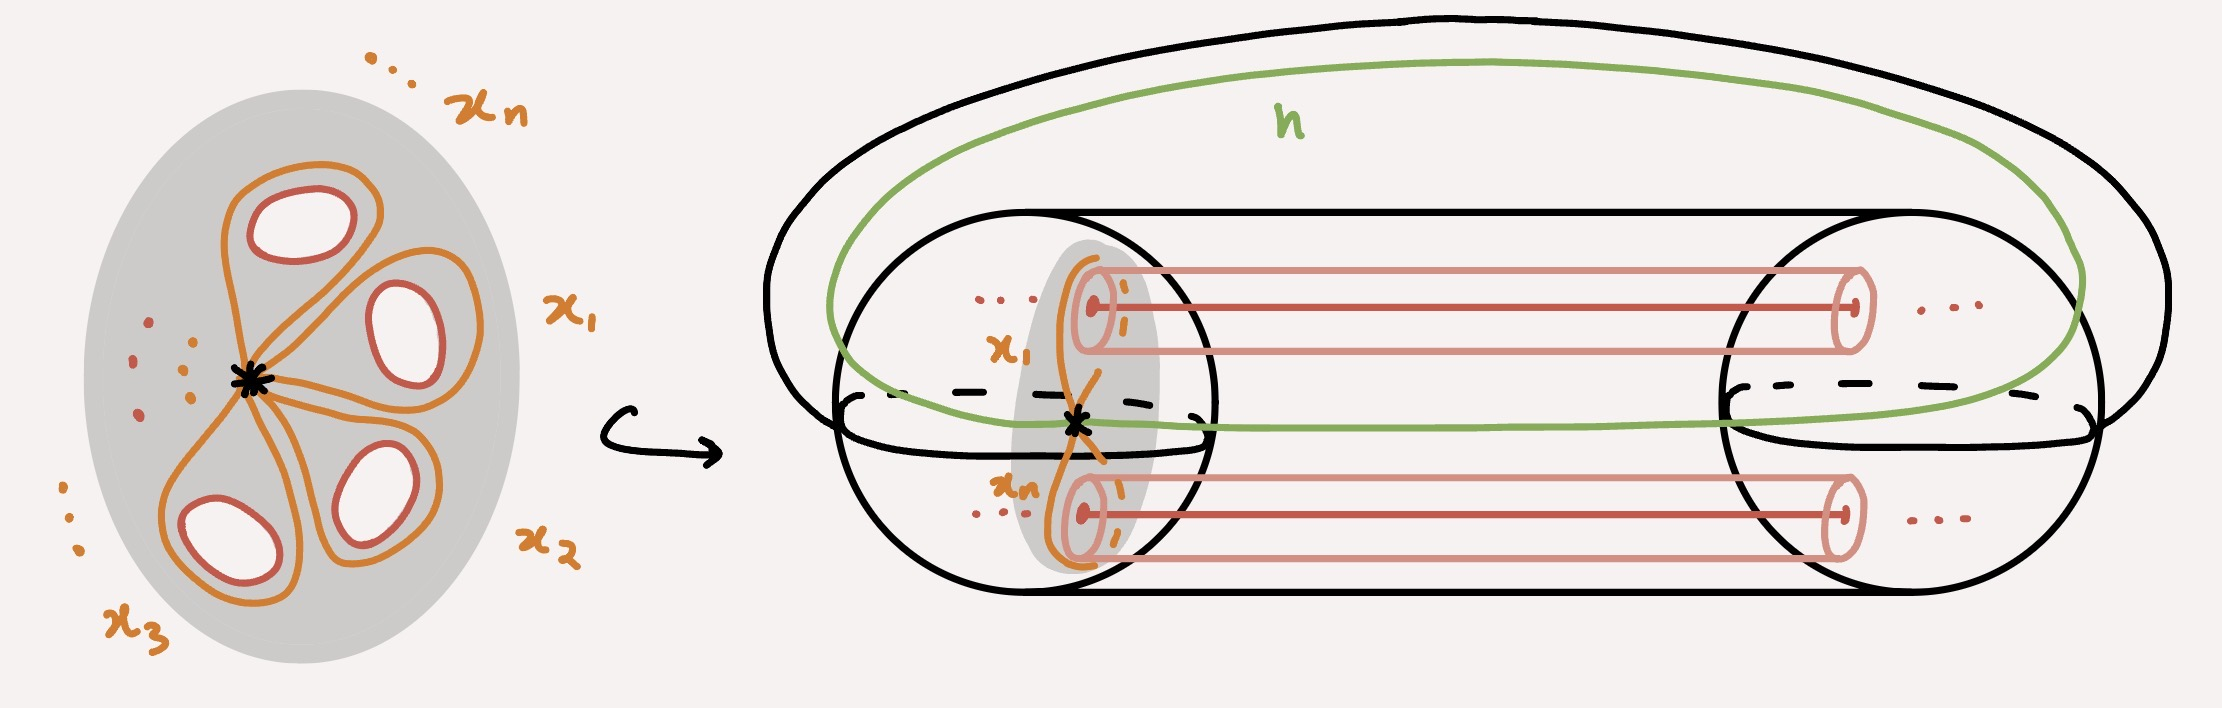
\includegraphics[width=0.85\linewidth]{figures/fig_lec19_generators.png}
\end{center}

To get the relations, check that
\begin{itemize}
\item the longitude commutes with each meridional generator, so $[x_i,h]=1$ for all $1\leq i\leq n$,
\item for each solid torus $S^1\times D^2$ we glue back in, $\mathrm{pt}\times\partial D^2$ gets attached along the $(p,q)$ torus knot, so $[\partial D^2] = x_i^{a_i}h^{b_i}=1$,
\item the product of all $x_i$'s is nullhomotopic, so $\prod_{i=1}^n x_i = 1$.
\end{itemize}

This gives the presentation for $\pi_1$:
\[
\pi_1(\Sigma(a_1,\dots,a_n)) \cong \left\langle x_1,\dots,x_n,h \,\Big|\, [x_i,h]=1,\ x_i^{a_i}h^{b_i}=1,\ \prod_{i=1}^n x_i = 1\right\rangle.
\]

Now, let's think about the character variety of this fundamental group. To each generator, we need to assign an element of $\SU(2)$, and this assignment must preserve the relations. We want to find irreducible representations, i.e., representations with the smallest possible stabilizer under conjugation. If a representation has a large stabilizer, then it's trivial, since for $\rho$ reducible, it factors through the abelianization, which is zero for homology spheres.

\begin{lemma}
If $\rho$ is irreducible, then $\rho(h)=\pm\mathrm{Id}$.
\end{lemma}

\begin{proof}
Assume not: $\rho(h)\neq\pm\mathrm{id}$. Then up to conjugation, $\rho(h)$ is a diagonal matrix:
\[
\rho(h) = \begin{pmatrix}e^{i\theta}&0\\0&e^{-i\theta}\end{pmatrix}, \qquad \theta\neq 0,\pi.
\]
One can check that the only elements in $\SU(2)$ which commute with a diagonal matrix are the elements in that $S^1$ subgroup: if
\[
\begin{pmatrix}\alpha & -\bar\beta\\ \beta & \bar\alpha\end{pmatrix}\begin{pmatrix}e^{i\theta} & 0\\ 0 & e^{-i\theta}\end{pmatrix} = \begin{pmatrix}e^{i\theta} & 0\\ 0 & e^{-i\theta}\end{pmatrix}\begin{pmatrix}\alpha & -\bar\beta\\ \beta & \bar\alpha\end{pmatrix},
\]
\[
\begin{pmatrix}\alpha e^{i\theta} & -\bar\beta e^{-i\theta}\\ \beta e^{i\theta} & \bar\alpha e^{-i\theta}\end{pmatrix} = \begin{pmatrix}\alpha e^{i\theta} & -\bar\beta e^{i\theta}\\ \beta e^{-i\theta} & \bar\alpha e^{-i\theta}\end{pmatrix},
\]
so $\beta e^{i\theta}=\beta e^{-i\theta}$ and $-\bar\beta e^{i\theta} = -\bar\beta e^{-i\theta}$, so $\beta=0$. Thus
\[
\begin{pmatrix}\alpha & -\bar\beta\\ \beta & \bar\alpha\end{pmatrix} = \begin{pmatrix}\alpha & 0\\ 0 & \bar\alpha\end{pmatrix}.
\]
Since $x_i$ commutes with $h$, this implies that $\rho(x_i)$ is in the same subgroup as $\rho(h)$, implying that $\rho$ is reducible. \qedhere
\end{proof}

So we may as well assume that $\rho(h)=\pm I$. Now, let's ask ourselves what $\rho(x_i)$ can be for each $i$. For each of the $2$ choices, $\rho(h)=I$ or $\rho(h)=-I$. Using the third relation, we have that
\[
\rho(x_i^{a_i}h^{b_i}) = \rho(1), \qquad \rho(x_i)^{a_i}\rho(h)^{b_i}=1, \qquad \rho(x_i)^{a_i}(\pm1)^{b_i}=1,
\]
\[
\rho(x_i)^{a_i} = (\pm1)^{-b_i}.
\]
Therefore $\rho(x_i)$ is a root of unity, so there is a discrete set of choices for the conjugacy class of $\rho(x_i)$. In particular, $\rho(x_i)$ is in the conjugacy class of a
\[
\begin{cases} a_i^{\text{th}} \text{ root of unity}, & \text{if } (\pm1)^{-b_i}=\mathrm{id},\\ 2a_i^{\text{th}} \text{ root of unity}, & \text{if } (\pm1)^{-b_i}=-\mathrm{id}.\end{cases}
\]

Having fixed the $(a_i,b_i)$'s, for each tuple of choices for the conjugacy classes of the $\rho(x_i)$, we only need to enforce the last relation: $\prod\rho(x_i)=\mathrm{Id}$. Another way of phrasing this constraint is: fix conjugacy classes $[\theta_i]$ for each $x_i$. Can we find $\rho(x_i)\in[\theta_i]$ such that $\rho(x_1)\cdots\rho(x_n)=\mathrm{Id}$?
\begin{center}
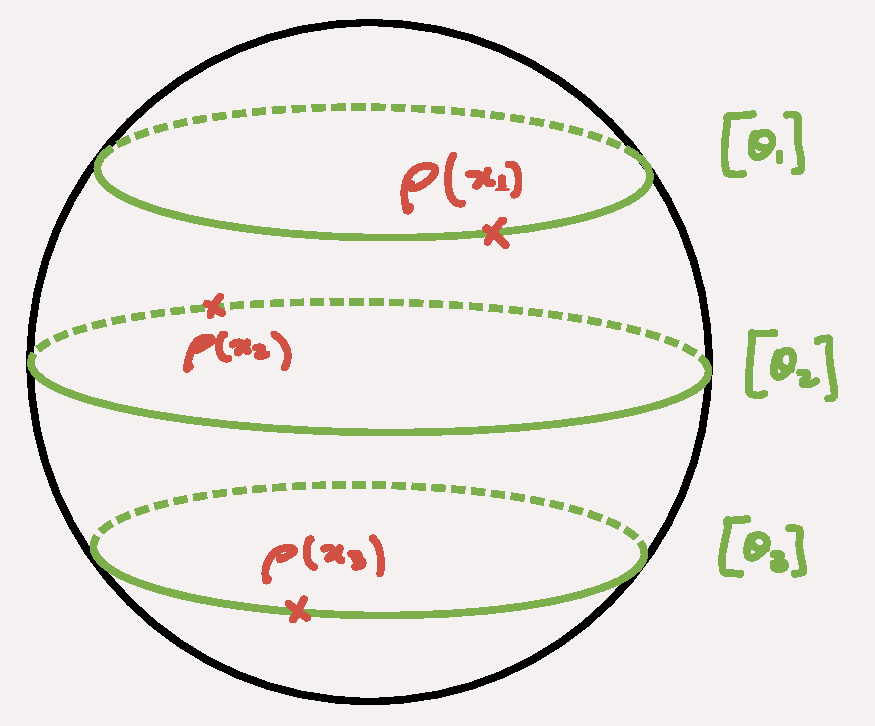
\includegraphics[width=0.3\linewidth]{figures/fig_lec19_rho_classes.png}
\end{center}

Let's now specialize to the case of $n=3$ singular fibres, $\mc{R}(\Sigma(a_1,a_2,a_3))$. The last relation becomes $x_1x_2=x_3^{-1}$. Since $\rho(x_3^{-1})$ is in the same conjugacy class as $\rho(x_3)$, $\rho(x_3)$ is in the conjugacy class of $\rho(x_1x_2)$. Up to conjugation, we can assume that $\rho(x_1)$ is in the right $S^1$ subgroup, e.g., is diagonal. Then, we can ask if
\[
\rho(x_1)\cdot[\theta_2]\cap[\theta_3]\neq\emptyset?
\]
\begin{center}
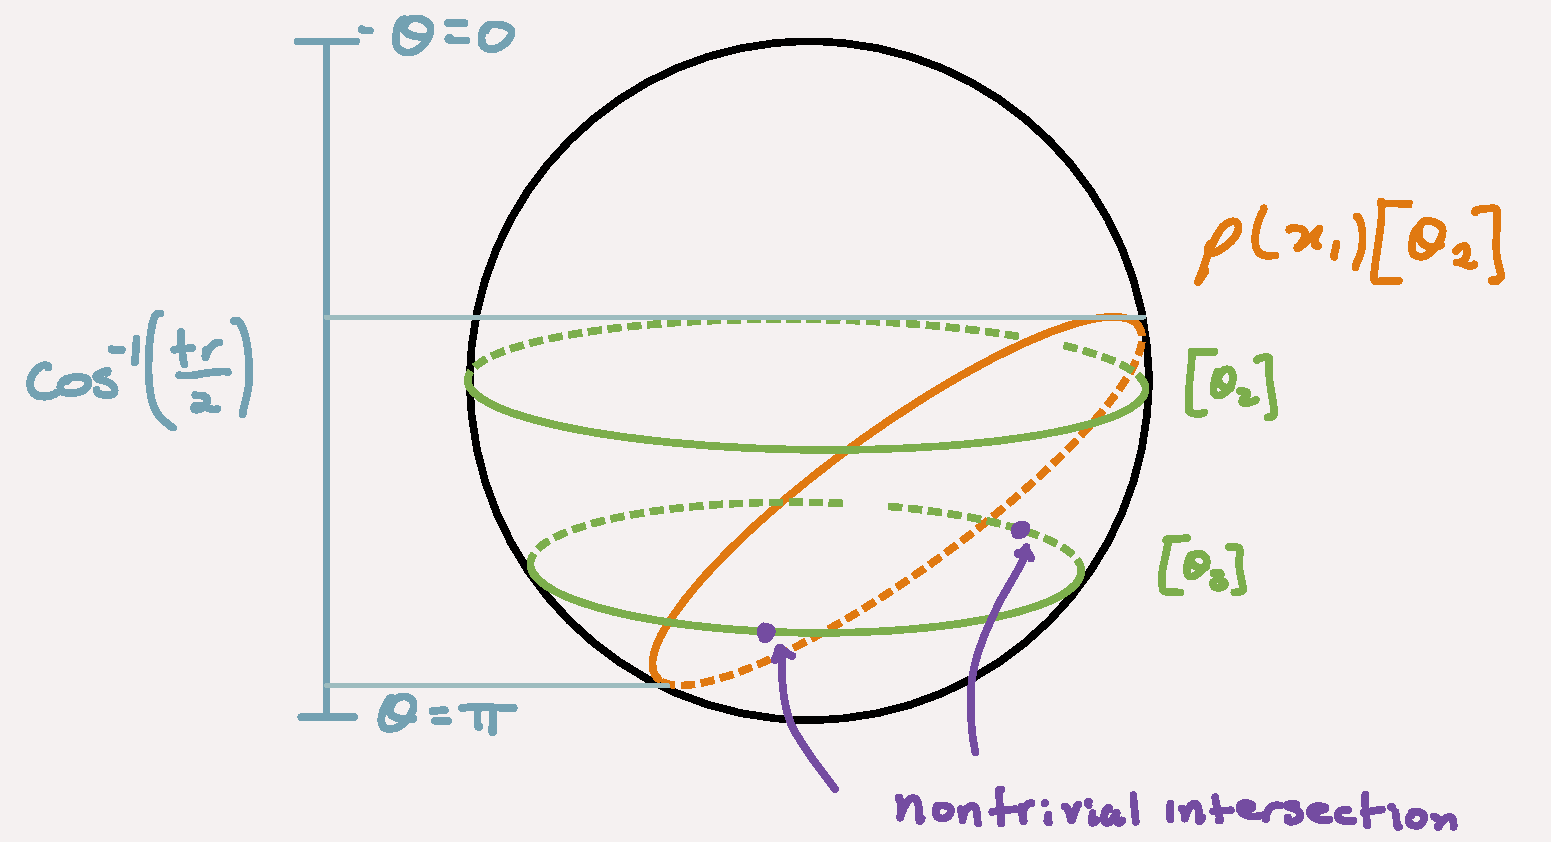
\includegraphics[width=0.55\linewidth]{figures/fig_lec19_intersection.png}
\end{center}

Since left multiplication by a fixed element of $\SU(2)$ is an isometry of $\SU(2)$, $\rho(x_1)[\theta_2]$ is another $S^2$ but it is slanted. To check whether it intersects with $[\theta_3]$, we can look at the range of values of $\cos^{-1}(\frac{1}{2}\mathrm{tr})$ on the $S^2$ given by $\rho(x_1)[\theta_2]$. Since the norm of matrices in $\SU(2)$ is $1$, the trace is minimized/maximized when the matrix is diagonal, so the endpoints must be at $|\theta_1-\theta_2|$ and $\theta_1+\theta_2$ (or, if $\theta_1+\theta_2>\pi$, $2\pi-(\theta_1+\theta_2)$).
\[
\begin{pmatrix}e^{i\theta_1}&0\\0&e^{-i\theta_1}\end{pmatrix}\cdot\begin{pmatrix}e^{-i\theta_2}&0\\0&e^{i\theta_2}\end{pmatrix} = \begin{pmatrix}e^{i(\theta_1-\theta_2)}&0\\0&e^{-i(\theta_1-\theta_2)}\end{pmatrix}
\]
\[
\begin{pmatrix}e^{i\theta_1}&0\\0&e^{-i\theta_1}\end{pmatrix}\cdot\begin{pmatrix}e^{i\theta_2}&0\\0&e^{-i\theta_2}\end{pmatrix} = \begin{pmatrix}e^{i(\theta_1+\theta_2)}&0\\0&e^{-i(\theta_1+\theta_2)}\end{pmatrix}
\]
Therefore $\cos^{-1}\left(\frac{\mathrm{tr}(A)}{2}\right)$ when $A\in\rho(x_1)[\theta_2]$ lies in the interval
\[
\left[|\theta_1-\theta_2|,\ \begin{cases}\theta_1+\theta_2 & \text{if } \theta_1+\theta_2\leq\pi\\ 2\pi-(\theta_1+\theta_2) & \theta_1+\theta_2>\pi\end{cases}\right].
\]
If $\theta_3$ is not in this interval, then we don't get a representation for that choice of conjugacy classes. If it does, then in general, the intersection $\rho(x_1)\cdot[\theta_2]\cap[\theta_3]$ will be a copy of $S^1$, since generally $S^1=S^2\cap S^2$ in $S^3$. But remember that we're quotienting by conjugation! We already quotiented a bit by choosing $\theta_1$ in the right $S^1$, but we can still conjugate within this $S^1$ and preserve the intersection. This $S^1$ is the ``leftover'' conjugation by the $S^1$ subgroup which contains $\rho(x_1)$. After doing so, for each $\{\theta_1,\theta_2,\theta_3\}$, we get one point in the character variety.

\begin{remark}
If the intersection is a point (instead of an $S^1$), this says that the leftover action fixes a point, which implies that the $x_i$ all commute, so $\pi_1$ is abelian and hence reducible.
\end{remark}

\begin{remark}
Since the $a_i$ are coprime, $\theta_3$ can never be at an end of the interval.
\end{remark}

Let's do an example for our favorite $3$-manifold so far: $\Sigma(2,3,5)$.

\textbf{Step 1:} Solve the equation $\left(\prod_{i=1}^3a_i\right)\left(\sum_{i=1}^3\frac{b_i}{a_i}\right)=1$:
\[
(2\cdot3\cdot5)\left(\frac{b_1}{2}+\frac{b_2}{3}+\frac{b_3}{5}\right) = 1, \qquad 15b_1+10b_2+6b_3=1.
\]
Notice: $15+6=21$, $10\cdot2=20$, $21-20=1$ $\Rightarrow$ $b_1=b_3=-1$, $b_2=2$ works.

\textbf{Step 2:} Compute $\pi_1$:
\[
\pi_1(\Sigma(2,3,5)) = \langle x_1,x_2,x_3,h \mid [x_i,h]=1,\ x_1^2=h,\ x_2^3=h^{-1},\ x_3^5=h^{-1},\ x_1x_2x_3=1\rangle.
\]

\textbf{Step 3:} Find representations which satisfy the first two relations:

If $\rho(h)=I$: $\rho(x_1)^2=\mathrm{Id}$ $\Rightarrow$ $\rho(x_1)=\pm\mathrm{Id}$ $\Rightarrow$ $\rho(x_2x_3)=1$ $\Rightarrow$ $\rho(x_2)\rho(x_3)=\pm\mathrm{Id}$ $\Rightarrow$ representation is reducible.

If $\rho(h)=-\mathrm{Id}$: $\rho(x_1)^2=-\mathrm{Id}$ $\Rightarrow$ $\rho(x_1)^4=\mathrm{Id}$ $\Rightarrow$ $\rho(x_1)$ is a $4^{\text{th}}$ root of unity whose square is $-1$ $\Rightarrow$ $\rho(x_1)\in[\pi/2]$.
\begin{align*}
\rho(x_2)^3 = -(-\mathrm{Id}) = \mathrm{Id} &\Rightarrow \rho(x_2)\in[\pi/3]\text{ or }[2\pi/3],\\
\rho(x_3)^5 = -(-\mathrm{Id}) = \mathrm{Id} &\Rightarrow \rho(x_3)\in[n\pi/5],\ n=1,2,3,4.
\end{align*}

\textbf{Step 4:} Use the range of $\rho(x_1)[\theta_2]$ to verify the last relation:

\textcolor{red}{\fbox{INSERT THIS STEP}}

It turns out that in general, the character variety for $n=3$ is a discrete set. Strictly speaking, this is still not enough to prove that no perturbation is needed (we still need to verify transversality, like in normal Morse theory) but in this case, everything works out. But it is true that if the character variety is not a discrete set, we definitely must perturb. Let's now take $n=4$, and show how $\mc{R}(\Sigma(a_1,a_2,a_3,a_4))$ need not be discrete.

Here it's the same story up until we get to the third condition. For each $4$-tuple of conjugacy classes $\{[\theta_1],[\theta_2],[\theta_3],[\theta_4]\}$, we ask if we can choose representatives in each class satisfying $x_1x_2x_3x_4=1 \iff x_1x_2 = x_4^{-1}x_3^{-1}$. As before, we formulate this as finding $\rho(x_1)\in[\theta_1]$ and $\rho(x_4^{-1})\in[\theta_4]$ such that
\[
\rho(x_1)[\theta_2]\cap\rho(x_4^{-1})[\theta_3]\neq\emptyset.
\]
To better visualize this condition, let's look at the image of stereographic projection $\pi : S^3\to\mathbb{R}^3$. Since $\pi$ is conformal, spheres get mapped to spheres. The size of each $[\theta_i]$ sphere is inversely proportional to $\theta_i$, and rotating $[\theta_2]$ by $\rho(x_1)$ corresponds to translating the center of $\pi([\theta_2])$ to lie at $\rho(x)\in\mathbb{R}^3$.
\begin{center}
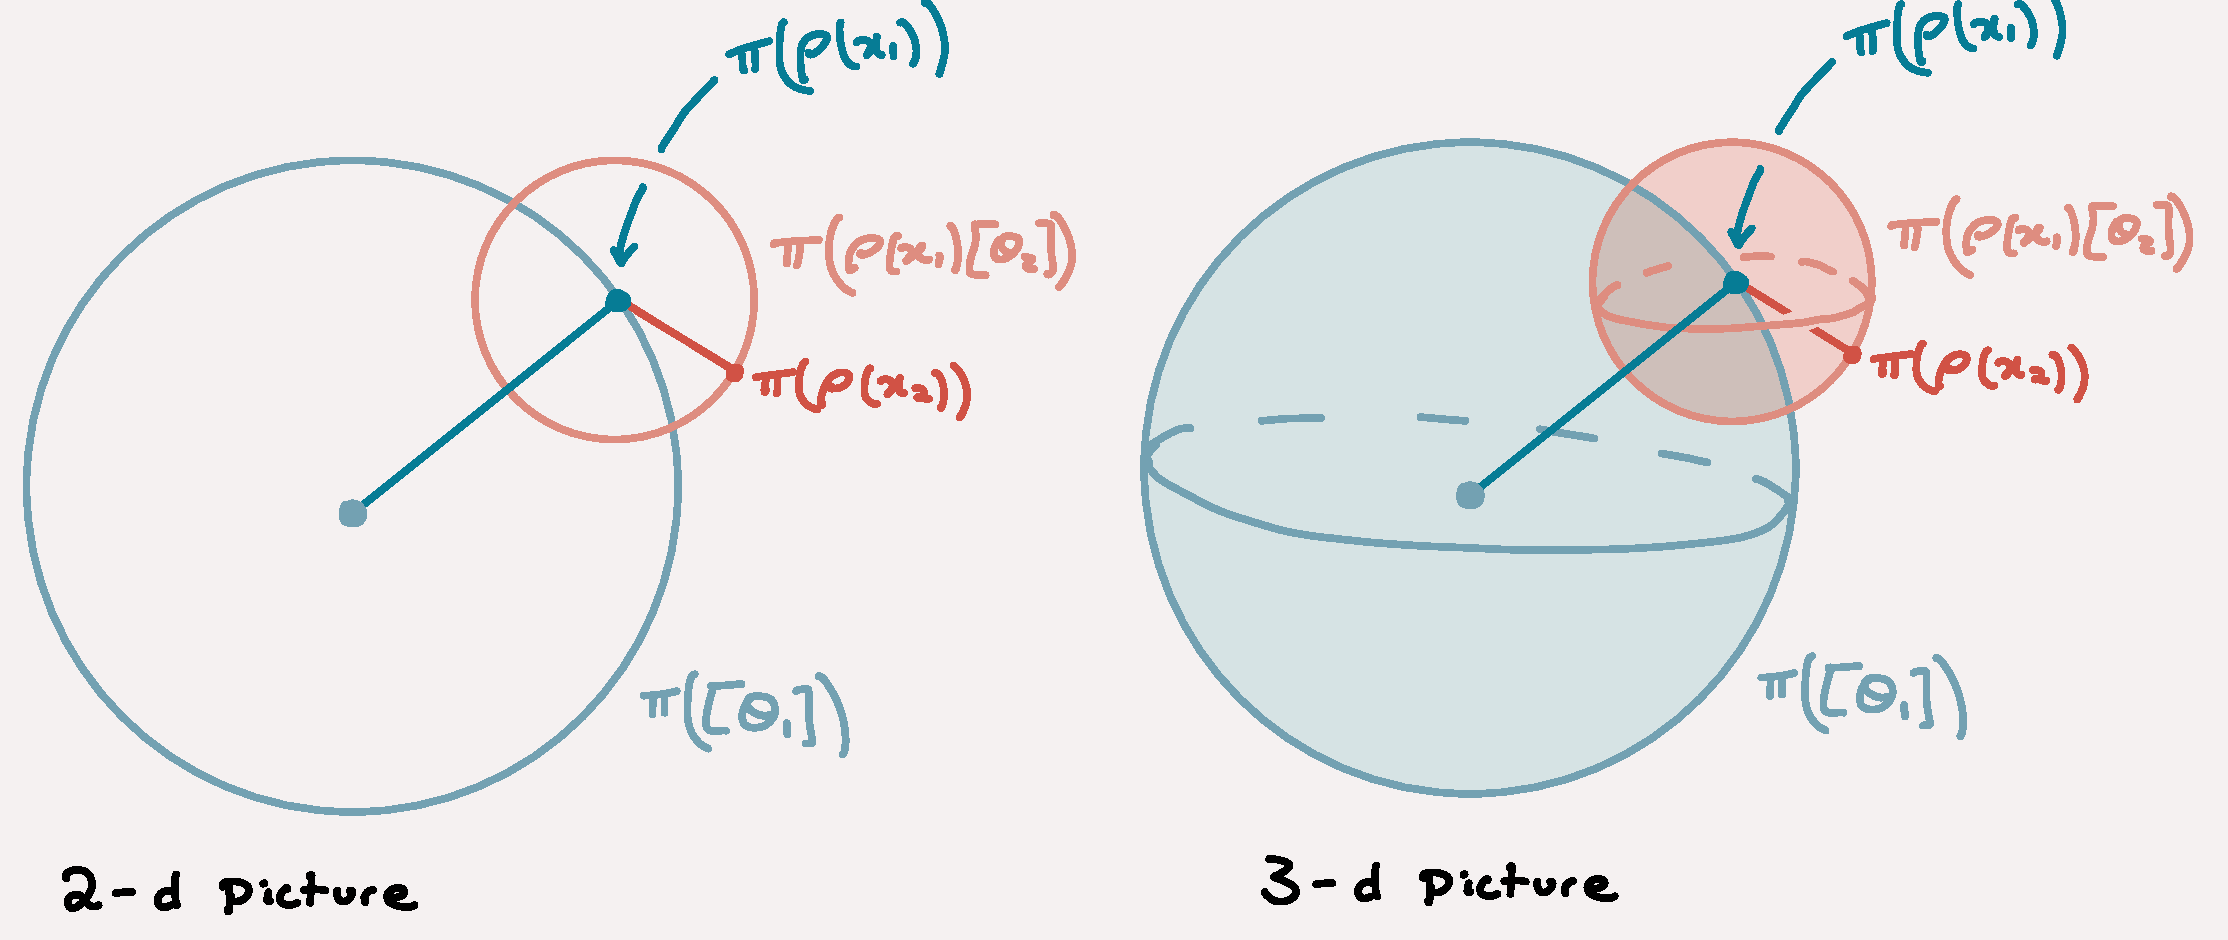
\includegraphics[width=0.9\linewidth]{figures/fig_lec19_stereographic.png}
\end{center}

However, trying to include the other two spheres makes this picture very busy! The relevant data is the radius of each sphere, and the location of the center-point of the subsequent sphere. So an even better way to visualize the condition that $x_1x_2x_3x_4=1$ is by a collection of four rigid rods whose lengths depend on $\theta_i$, where the start of rod $i$ is attached to the end of rod $i-1$. Then $x_1x_2x_3x_4=1$ exactly when the rods form a closed polygon in $\mathbb{R}^3$.
\begin{center}
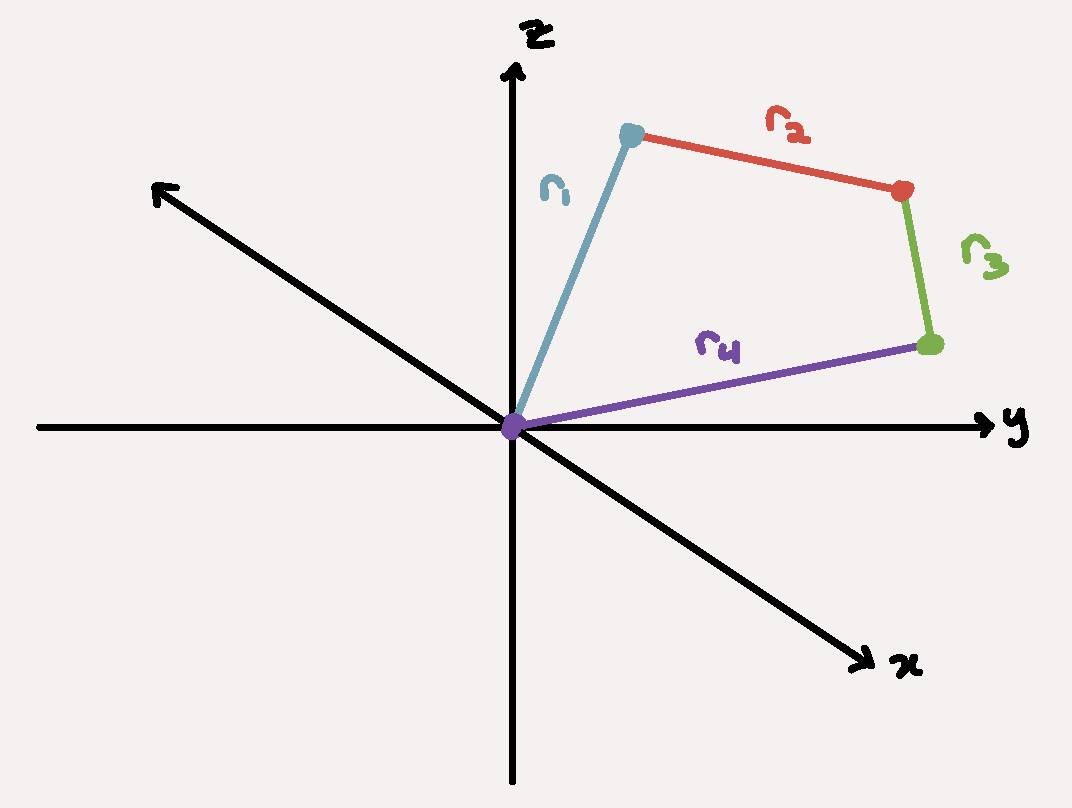
\includegraphics[width=0.4\linewidth]{figures/fig_lec19_rod_polygon.png}
\end{center}

In general, such a configuration of rods for a given set of side lengths does exist. The question then becomes how many are there, up to conjugation. The conjugation action is that of $\SU(2)$ acting on $\mathbb{R}^3$, so by rotations. We may first move $r_1$ to align with the $z$-axis. This is the same thing as conjugating to turn $\rho(x_1)$ into a diagonal matrix. The leftover action corresponds to rotating about the $z$-axis, since that fixes $\rho(x_1)$. Therefore we can rotate such that $r_2$ lies in the right-hand side of the $y$-$z$ plane.

\begin{center}
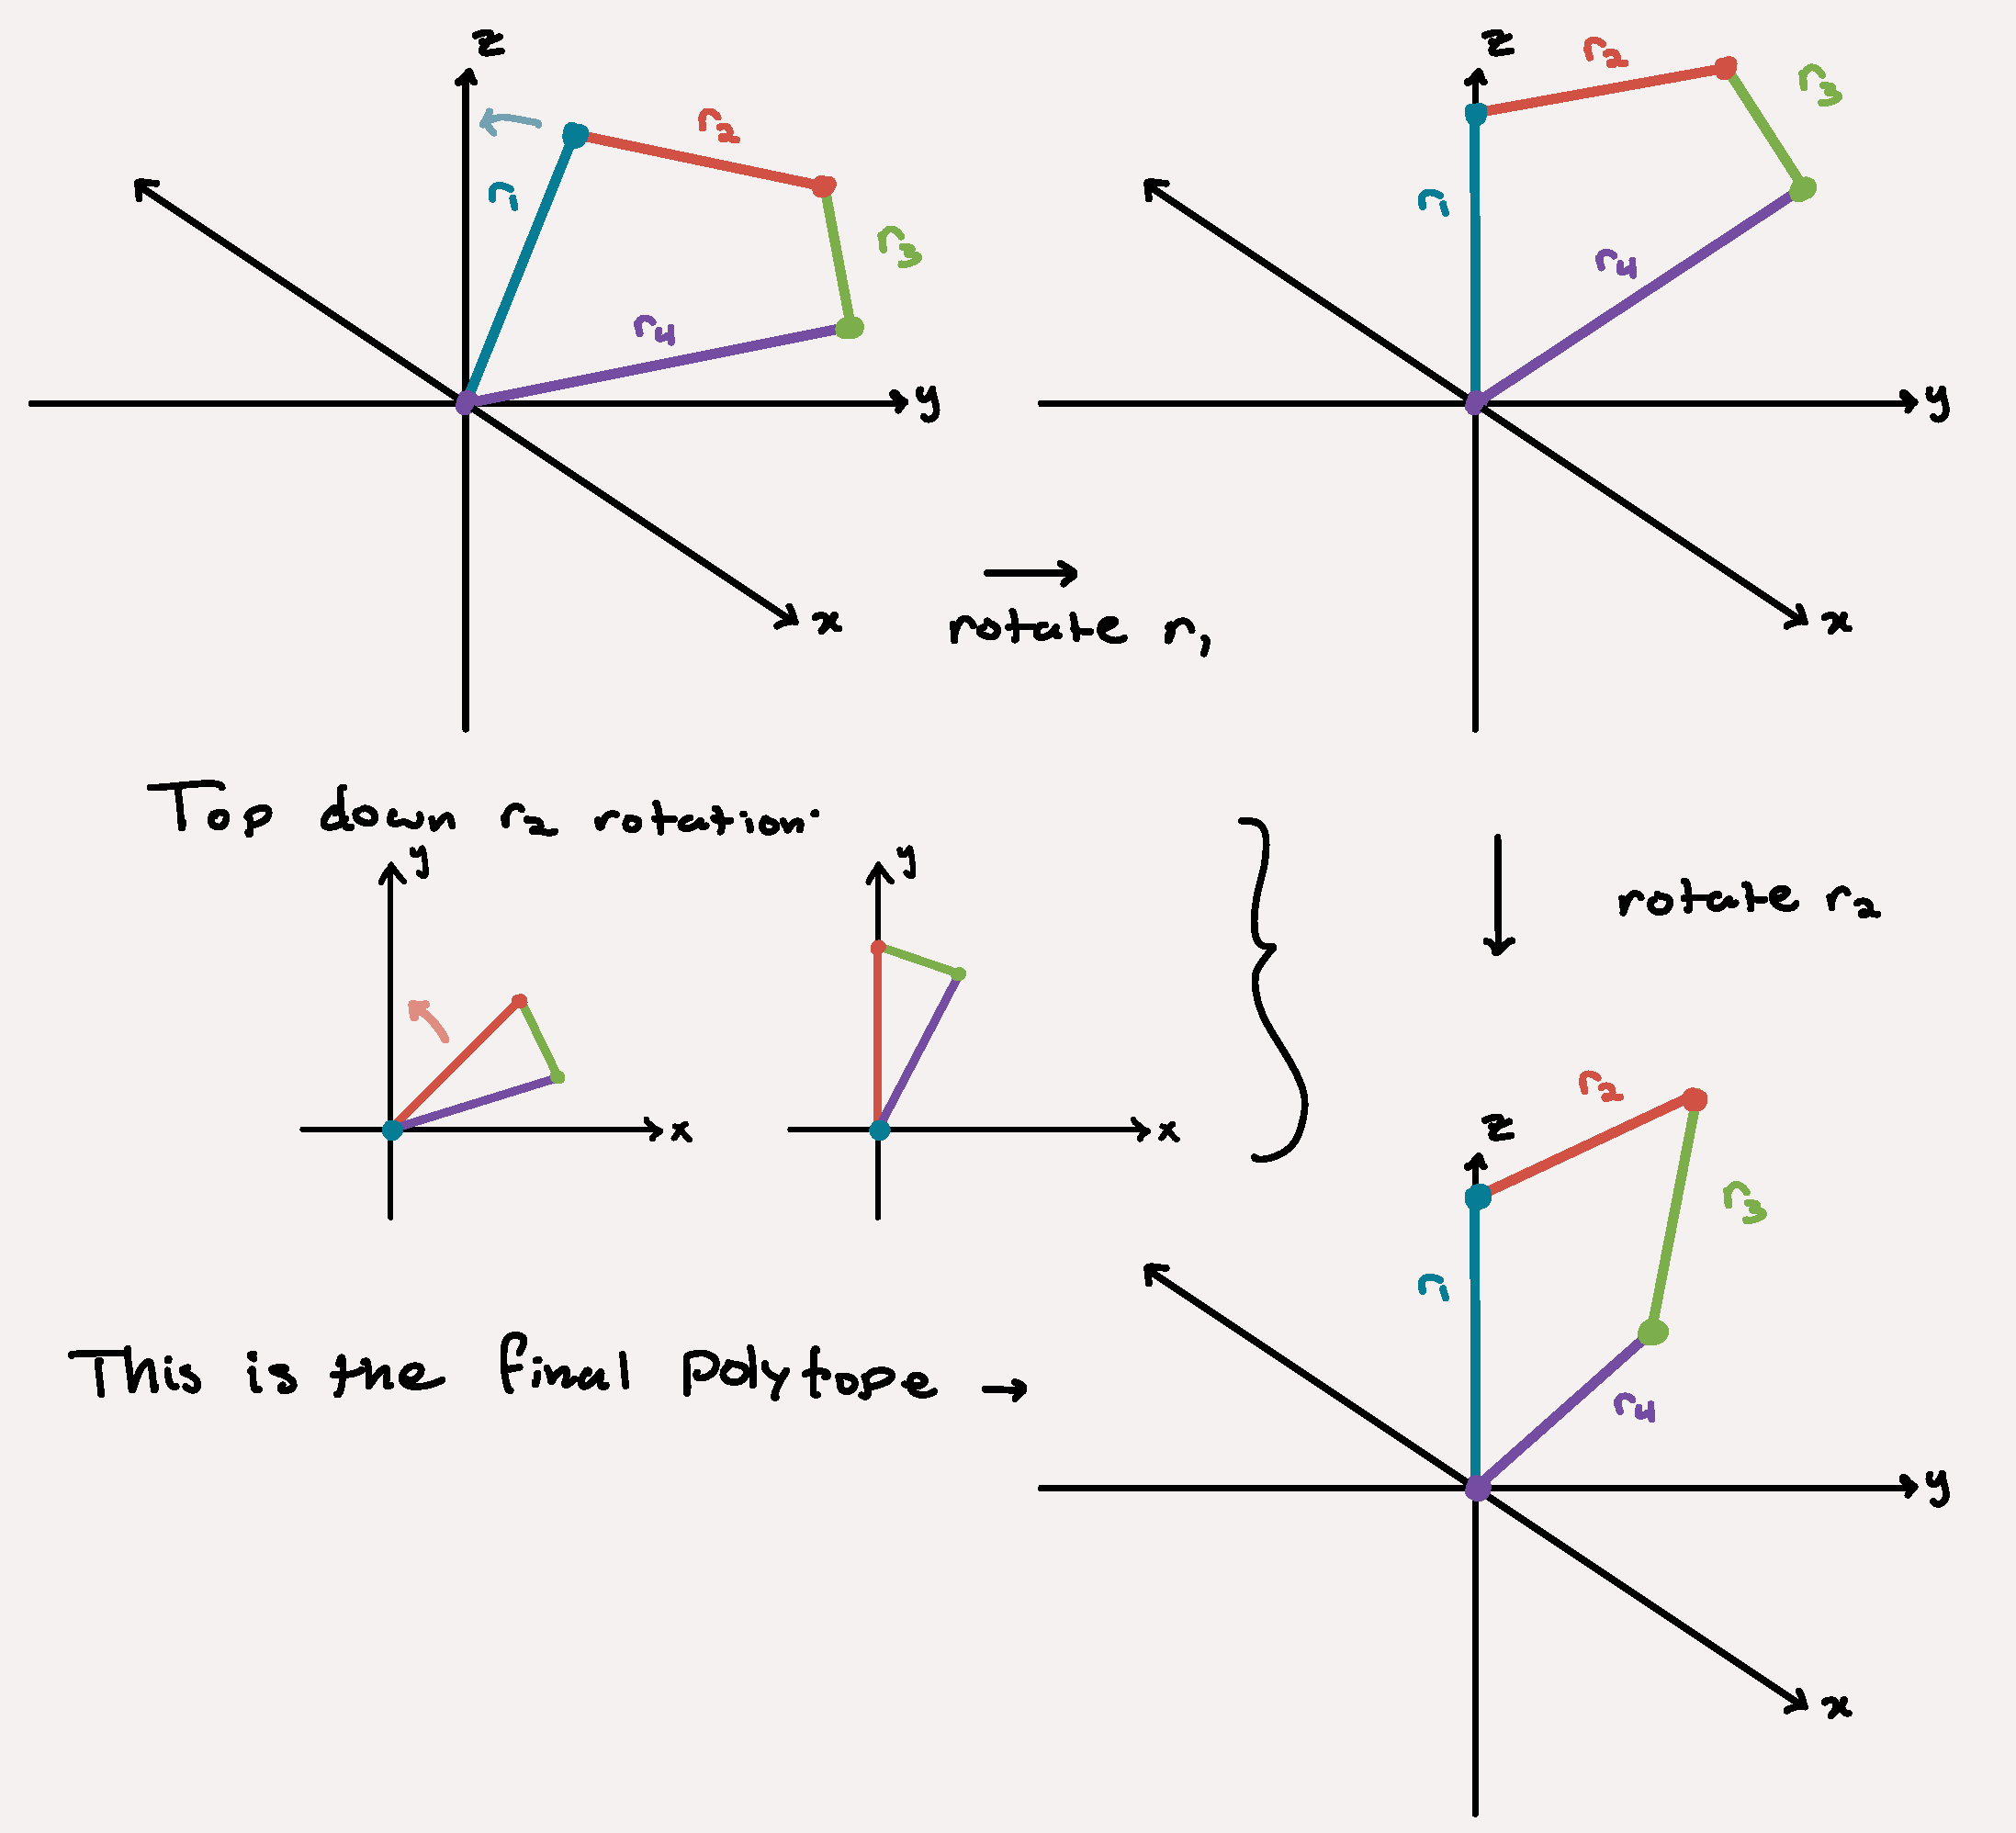
\includegraphics[width=0.9\linewidth]{figures/fig_lec19_rotations.png}
\end{center}

However, there is still an $S^1$ action on this polytope which is not given by conjugation. In fact, this $S^1$ action is a slice of a residual $S^2$'s worth of action in $\mc{R}$. This $S^2$ can be thought of as the double cone on $S^1$, where the cone points are the degeneration of the symmetry due to the angle between $r_1$ and $r_2$, and $r_3$ and $r_4$.
\begin{center}
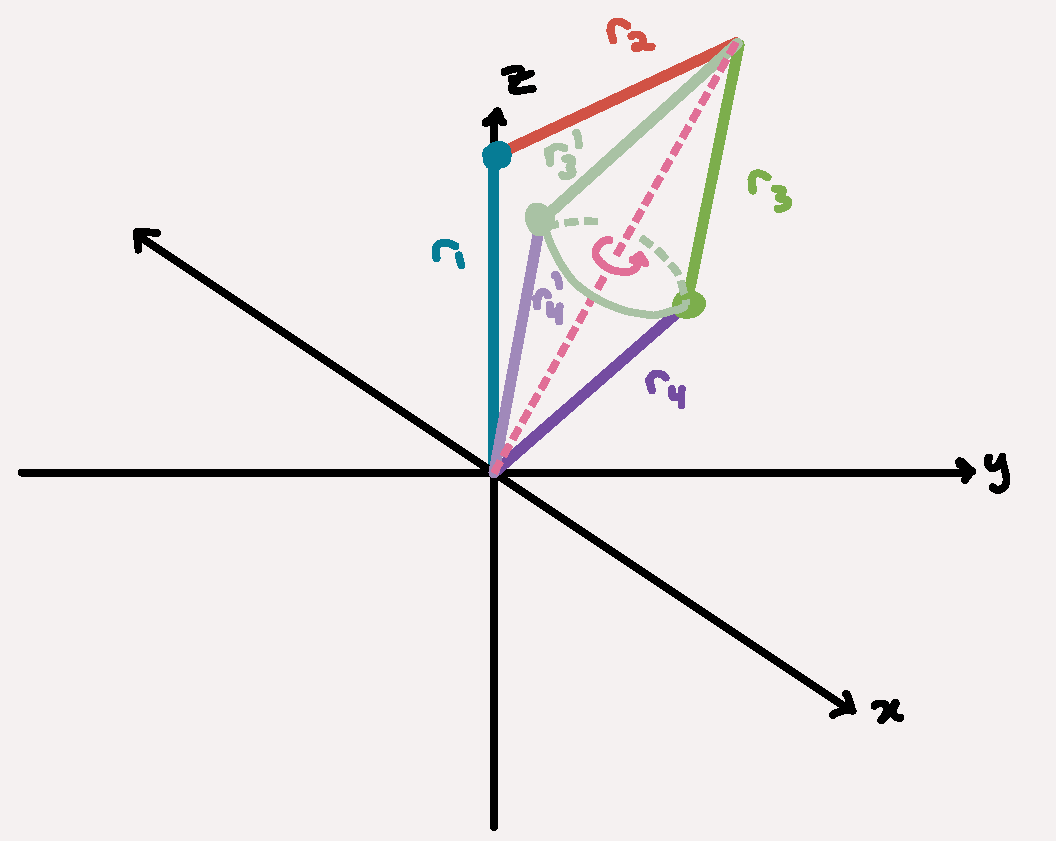
\includegraphics[width=0.35\linewidth]{figures/fig_lec19_s1_action.png}
\end{center}
\begin{center}
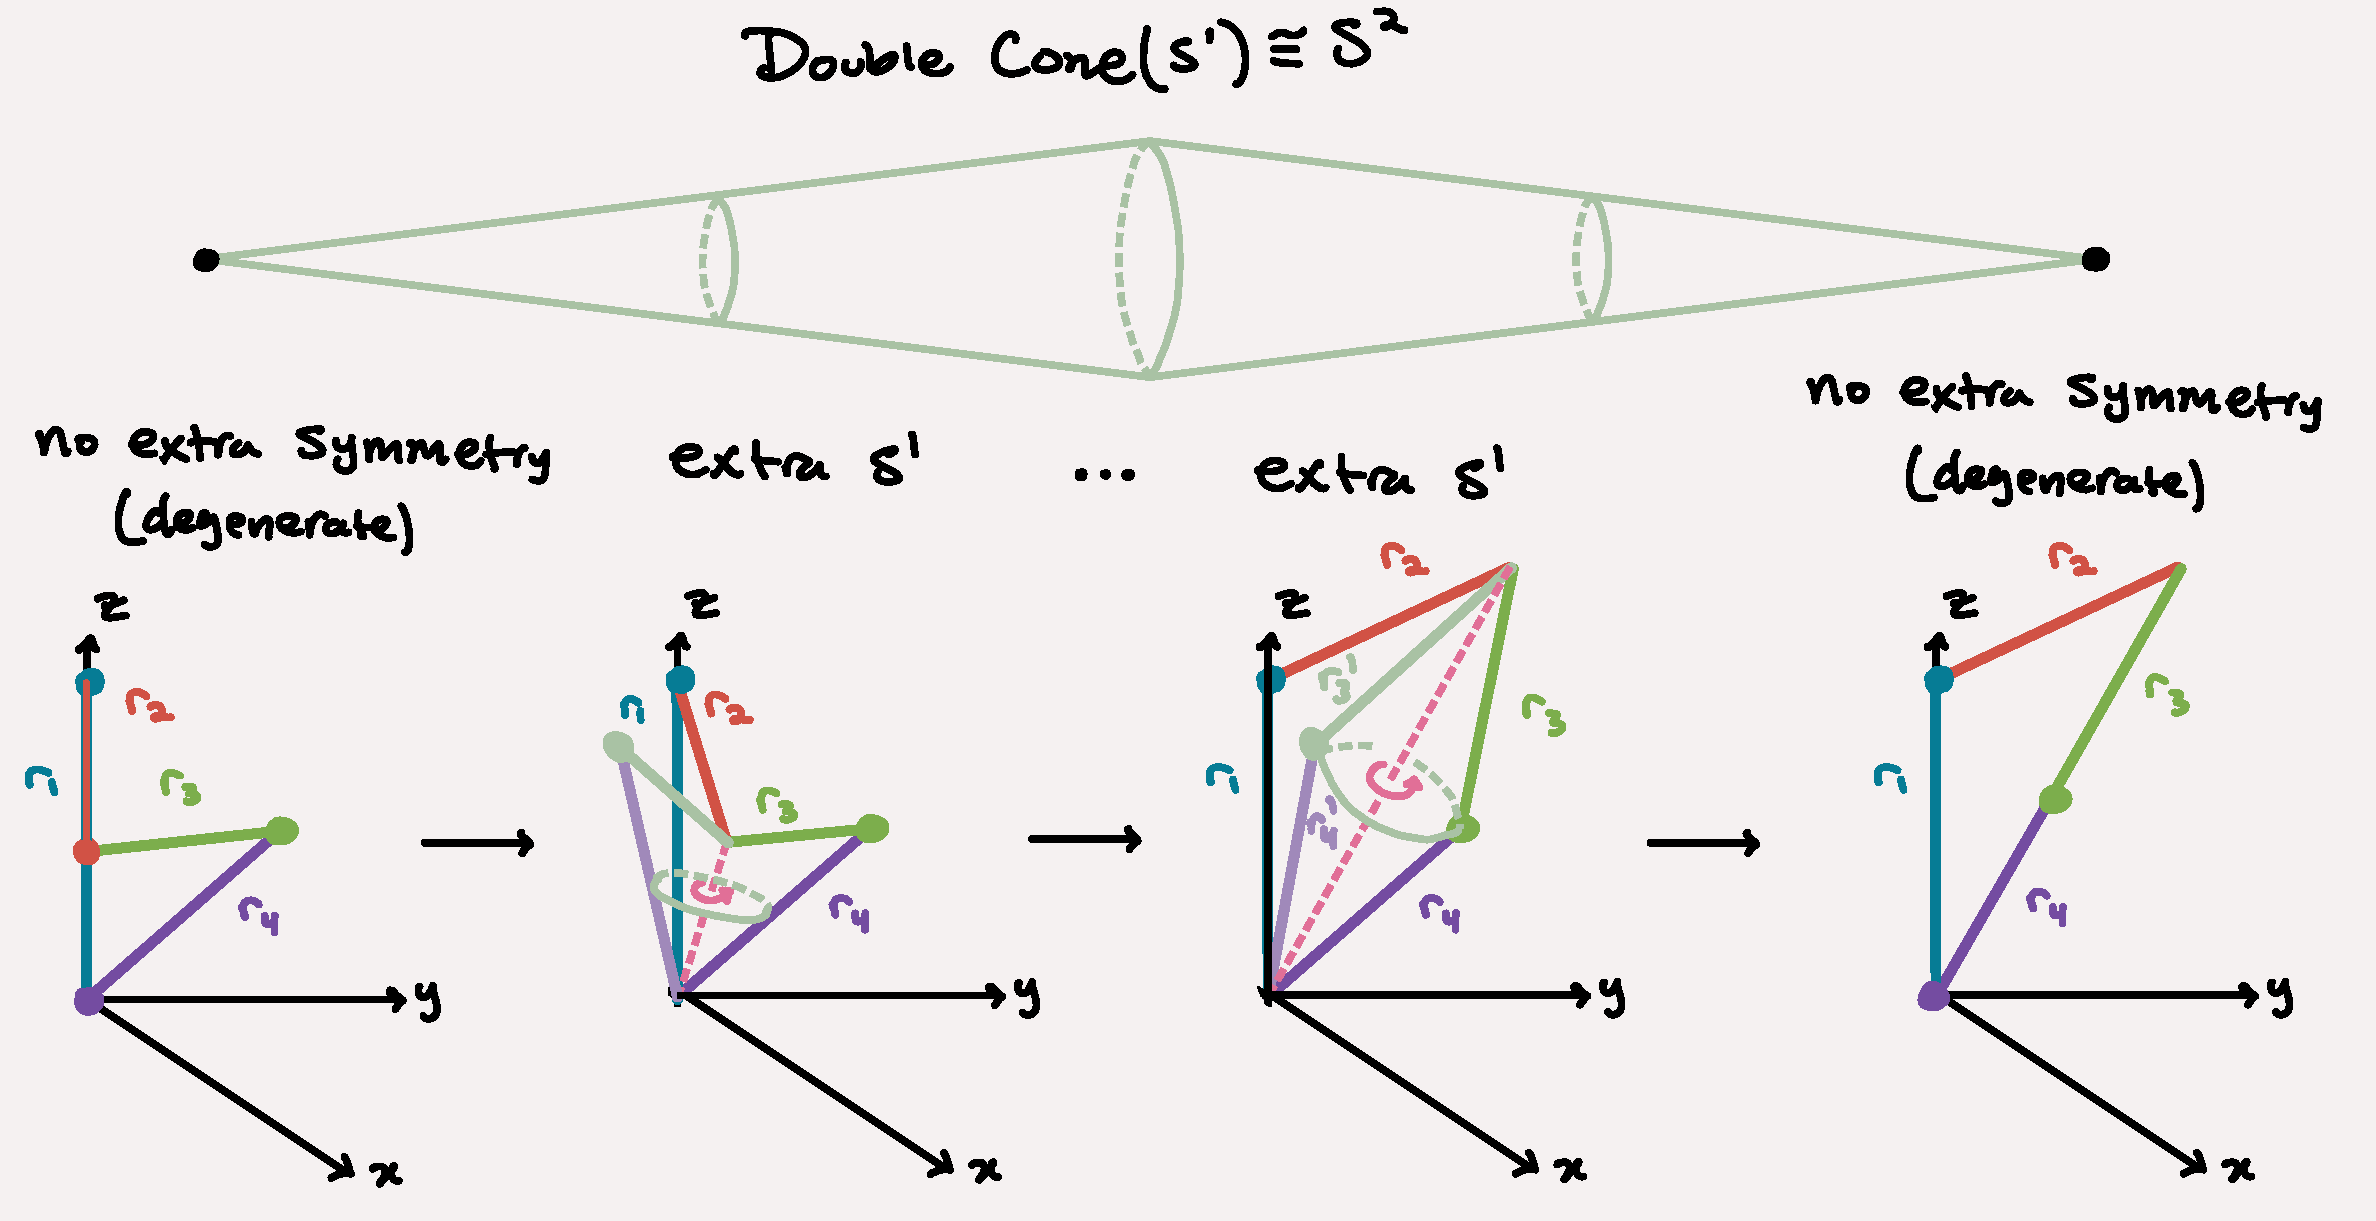
\includegraphics[width=\linewidth]{figures/fig_lec19_double_cone.png}
\end{center}

\end{document}
